\documentclass{ctexart}


\author{李约瀚 \\ 14130140331 \\ qinka@live.com \\ qinka@qinka.pw}
\title{FPGA设计基础实验报告 (一)}

\usepackage{listings}

%\lstset{frame=single,breaklines,numbers}

\begin{document}
    
        % Cover
        \thispagestyle{empty}
        \begin{center}
            \vspace*{4em}
            {\Huge\textbf{FPGA设计基础实验报告\\\vspace*{0.5em} (一)}}
            \vfill
            \begin{tabular}{c@{:}l}
                班级 & 1413014 \\
                学号 & 14130140331 \\ 
                姓名 & 李约瀚 \\ 
                教师 & 沈沛意 \\
            \end{tabular} 
            \vspace*{4em}\\
        \end{center}
        \newpage
        
       
        % Setting
        \setcounter{page}{0}
        \setcounter{section}{0}
        %\renewcommand\thesection{实验编号 1-\numeric{section} 题目: }
        %\renewcommand\thesubsection{}
        %\renewcommand\thesubsubsection{(\numeric{subsubsection})}

        %% Exp 1-1
        \section{控制二极管循环发光}
        
        \subsection{实验目的}
        \begin{enumerate}
        \item 熟悉 ISE 软件,会使用ISE软件进行设计和仿真
        \item 学会程序下载
        \end{enumerate}

        \subsection{实验内容}

        \begin{enumerate}
        \item 创建工程
        \item 设计输入
        \item 综合实现
        \item 进行硬件配置
        \end{enumerate}

        \subsection{报告正文}

        \subsubsection{实验原理}
        
        根据 Nexys3 的指引手册,Nexys3 开发板上有8个并排放置的发光二极管,从左到右分别标注的是LD0~LD7,
        实验要求其中一个二极管发光,其他7个二极管均处于截止状态。二极管发光的顺序按照向左或者向右的方向,并有波动开关SW0控制方向。
        
        \subsubsection{实验过程}

        \paragraph{新建工程}

        打开 ISE 14.7之后,选择新建工程,将工程的路径设置好。
        在单击下一步之后,选择 Nexys3 的 Spartan6 XC6SLX16-CS324 芯片对应的配置。硬件描述语言选择 Verilog,其中的设计硬件用的描述语言是 Verilog。
        然后点击下一步之后进入工程信息页面并确认无误之后,点击完成结束工程的创建。

        \paragraph{设计输入}

        在菜单 \verb|Project| 中选择 \verb|New Source| 创建新的设计,并选择 \verb|Verilog Module| 创建文件。
        
        其中输入的设计文件是
\begin{lstlisting}[language=Verilog]
`timescale 1ns / 1ps
// Copyright (C) Xilinx
module led_shift(
input clk,
input reset,
input dir_r_l,
output [7:0] led
);

reg [7:0] led;
reg [28:0] cnt;	//计数分频器
always @ (posedge clk or posedge reset) begin
if(reset) begin
cnt <= 29'd0;
end
else begin
if(cnt == 29'd99_999_999) begin
cnt <= 29'd0;
end
else begin
cnt <= cnt + 1;
end
end
end

reg new_second;	//得到一秒的信号
always @ (posedge clk or posedge reset) begin
if(reset) begin
new_second <= 1'b0;
end
else begin
if(cnt == 29'd99_999_999) begin
new_second <= 1'b1;
end
else if(new_second) begin
new_second <= 1'b0;
end
end
end

//控制二极管循环发光
always @ (posedge clk or posedge reset) begin
if(reset) begin	
led <= 8'b0000_0001;
end
else begin
if(new_second) begin
if(dir_r_l == 1'b1) begin	//向右移动
led <= {led[0], led[7:1]};
end
else begin	//向左移动
led <= {led[6:0], led[7]};
end
end
end
end

endmodule
\end{lstlisting}

        \paragraph{综合与实现}

		在左侧的 \verb|Design| 面板中下方中 双击 \verb|Synthesize-XST| 开始综合过程。
		

        在左侧的 \verb|Design| 面板中的 \verb|Hierarchy| 中选中创建的 HDL 源文件,在下方的双击 \verb|View RTL Schematic| 查看电路。

        \begin{figure}
\centering
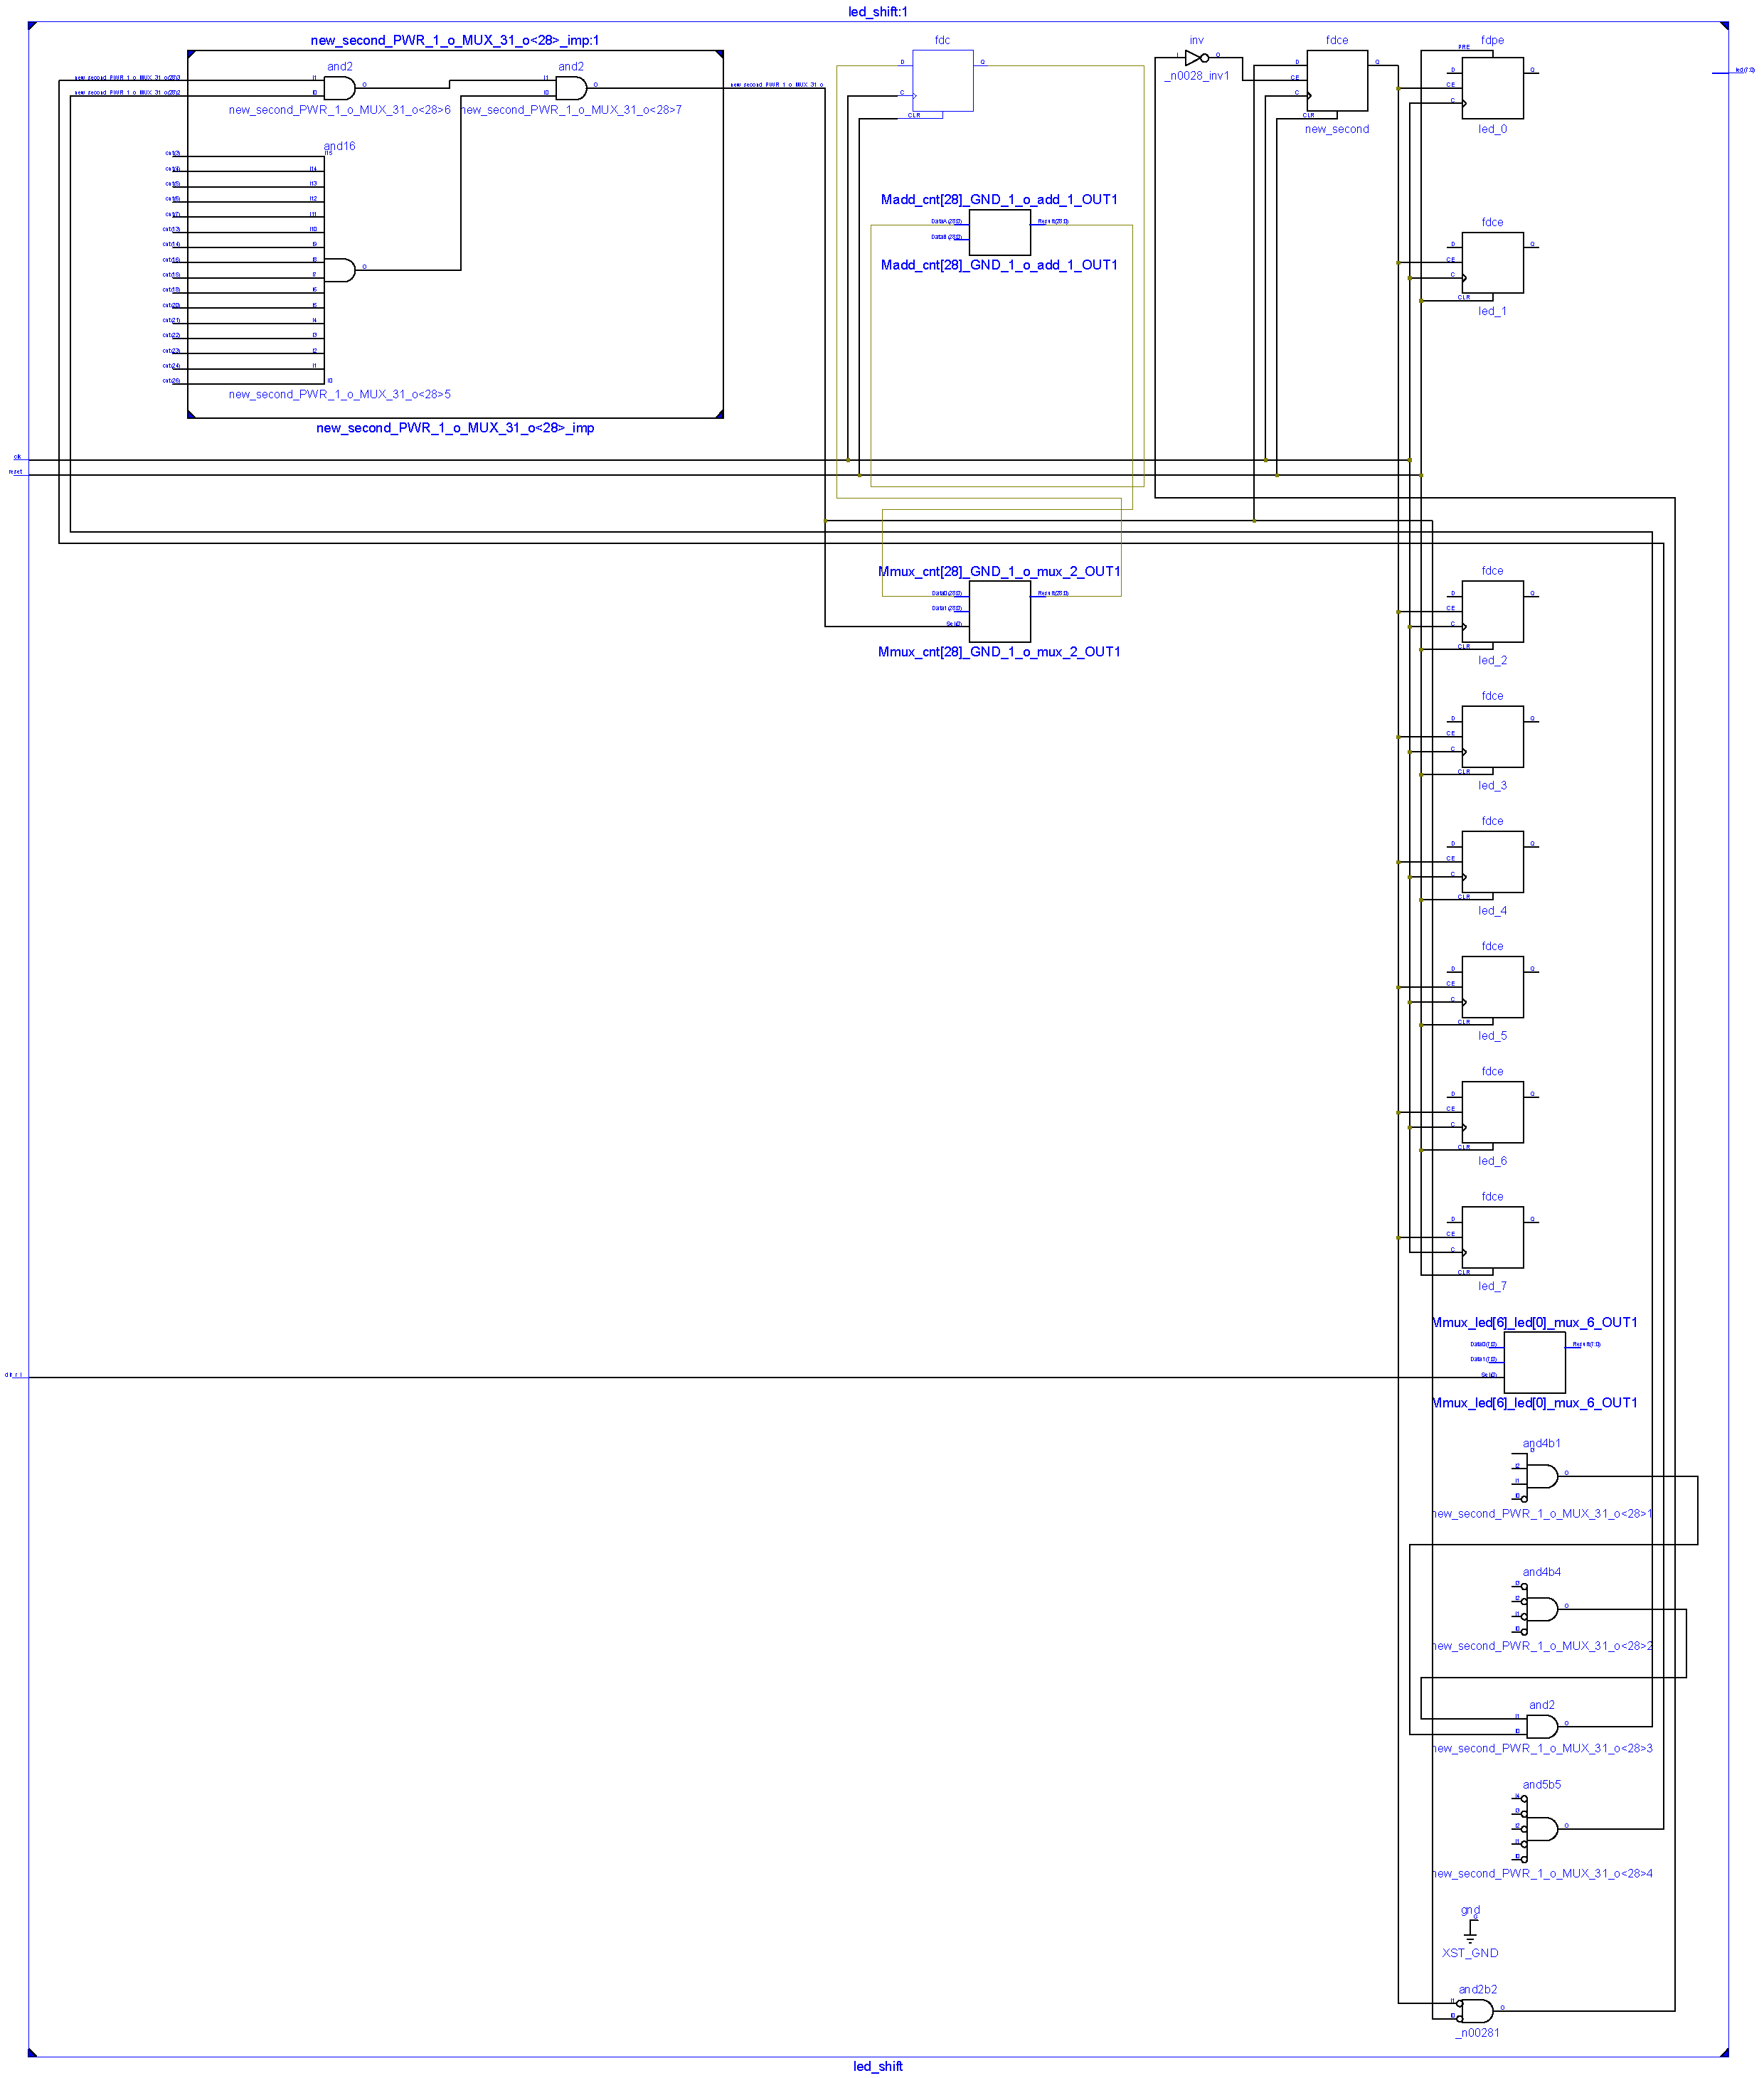
\includegraphics[width=1\linewidth]{report1-circiut-1.jpg}
\caption[Circuit]{}
\label{fig:report1-circiut-1}
\end{figure}

        之后添加用户约束文件,这个文件使得器件脚针与外围设备可以绑定,链接。
        添加的方式可以在 \verb|Design| 面板中找到 带有 \verb|Pre| 前缀的 \verb|PlanAhead| 中配置脚针。或者为工程添加用户约束文件。
		
        \begin{figure}
\centering
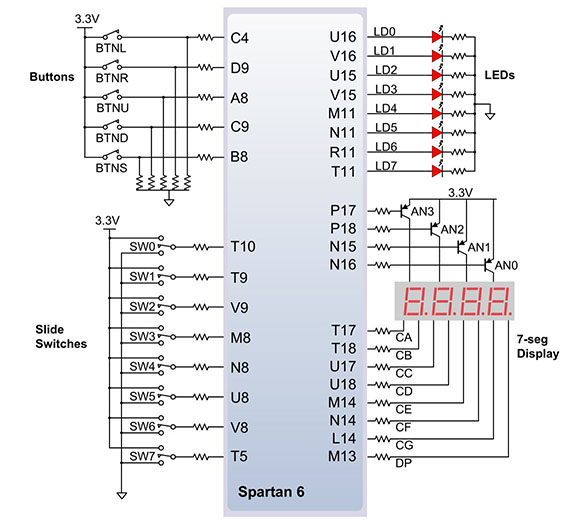
\includegraphics[width=1\linewidth]{report-1-io-ports}
\caption{}
\label{fig:report-1-io-ports}
\end{figure}

        
        用户约束文件的内容大致是配置脚针(site) 与外围设备的链接配置。
\begin{lstlisting}
Net "clk"      LOC = V10;
Net "reset"  LOC = C9;
Net "dir_r_l" LOC = T10;
Net "clk"      IOSTANDARD = LVCMOS33;
Net  "reset" IOSTANDARD = LVCMOS33;
Net "dir_r_l" IOSTANDARD = LVCMOS33;

Net "led[0]" LOC = U16;
Net "led[1]" LOC = V16;
Net "led[2]" LOC = U15;
Net "led[3]" LOC = V15;
Net "led[4]" LOC = M11;
Net "led[5]" LOC = N11;
Net "led[6]" LOC = R11;
Net "led[7]" LOC = T11;
Net "led[0]" IOSTANDARD = LVCMOS33;
Net "led[1]" IOSTANDARD = LVCMOS33;
Net "led[2]" IOSTANDARD = LVCMOS33;
Net "led[3]" IOSTANDARD = LVCMOS33;
Net "led[4]" IOSTANDARD = LVCMOS33;
Net "led[5]" IOSTANDARD = LVCMOS33;
Net "led[6]" IOSTANDARD = LVCMOS33;
Net "led[7]" IOSTANDARD = LVCMOS33;
\end{lstlisting}
		
        然后执行的步骤是实现。这个步骤中会执行翻译、映射、与布局布线。双击
        \verb|Implement Design| 自动执行上述步骤。
		
        \paragraph{器件配置}

        配置器件之前首先需要进行的是生成对应的配置文件。在 \verb|Design| 面板中
        的 \verb|Generate Programming File|  双击之后会自动生成 二进制比特的配置文件。
        之后将开发版通过USB链接到电脑后。双击 \verb|Configure Target Device| 配置设备。

        对FPGA配置编程的时候,会打开一个窗口,初始化链之后可添加设备。然后将生成的配置文件写入
        FPGA 中。然后就测试 FPGA 控制 二极管发光的实际效果了。

        \begin{figure}
\centering
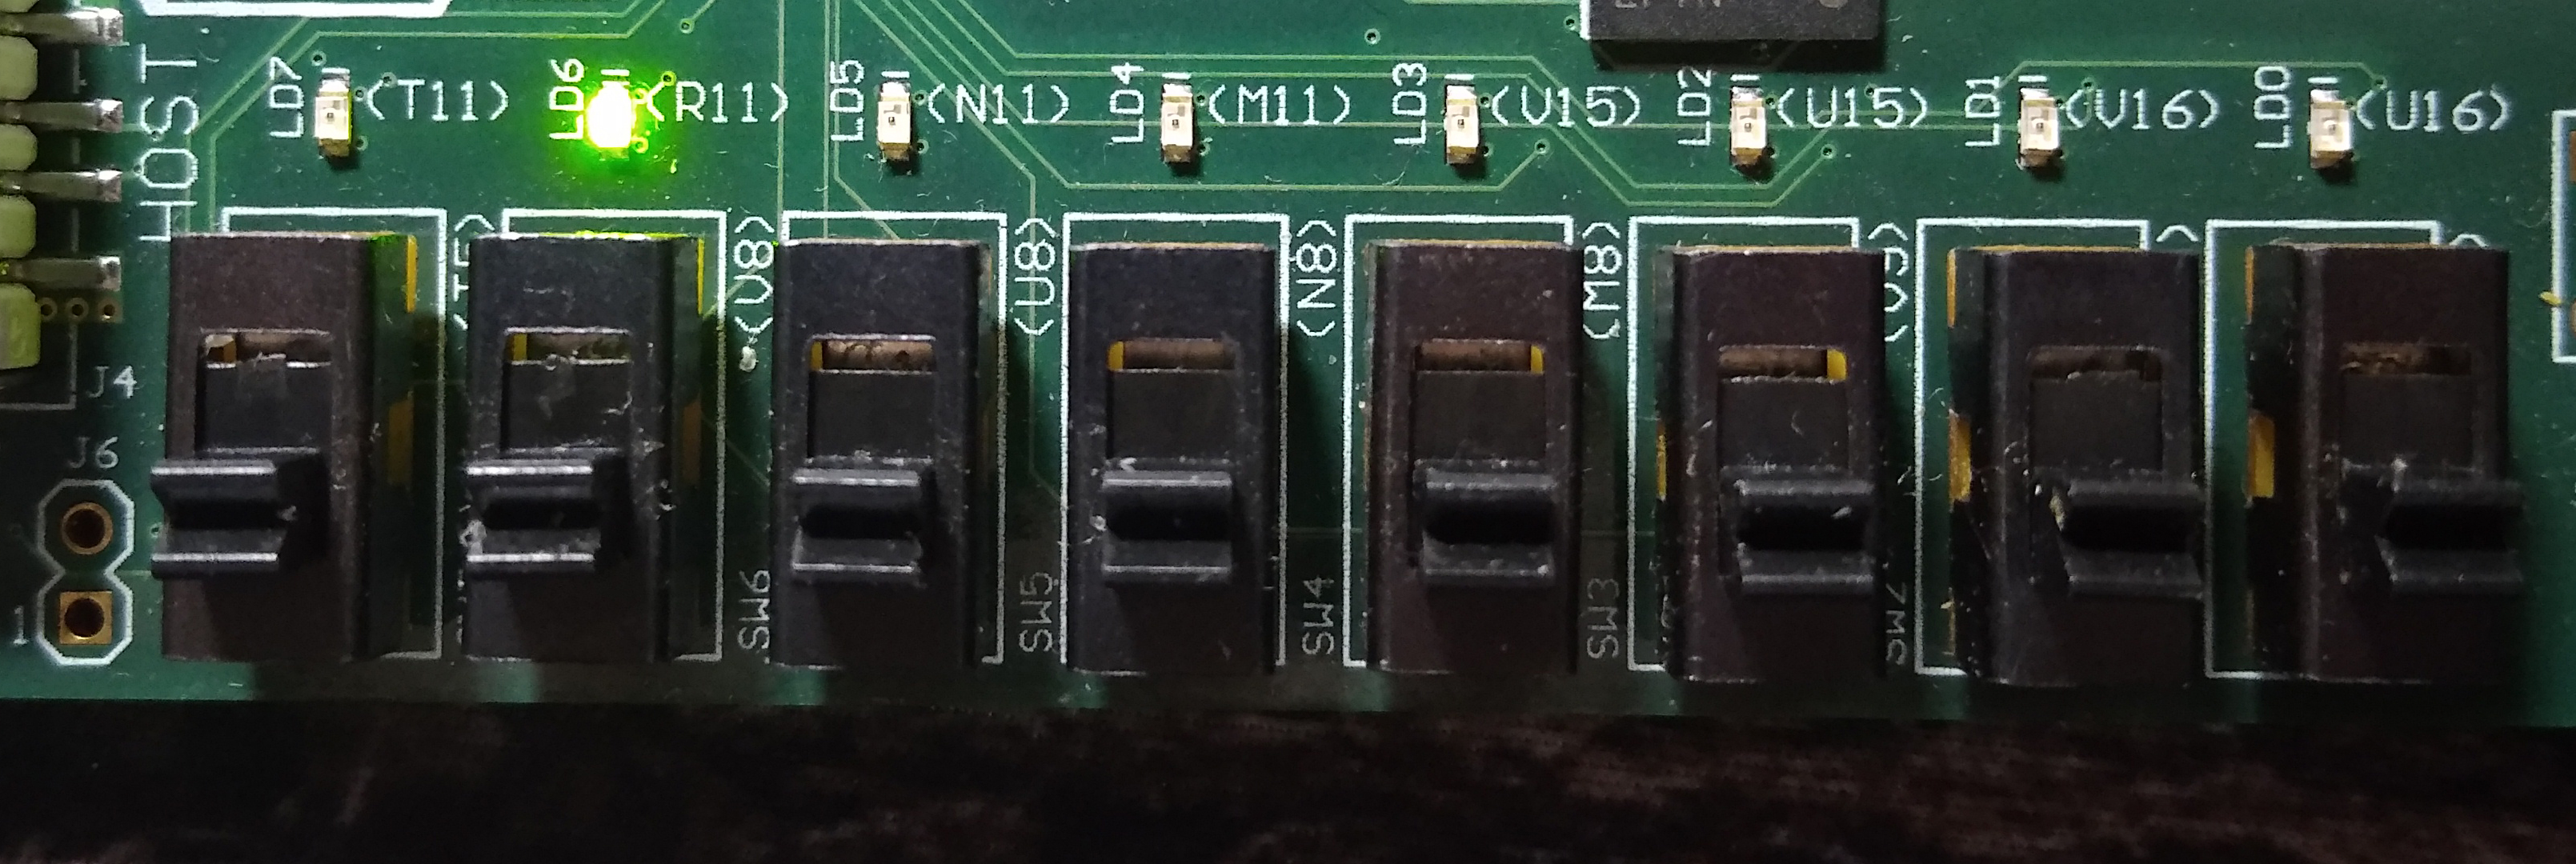
\includegraphics[width=1\linewidth]{report-1-rt-1}
\caption{}
\label{fig:report-1-rt-1}
\end{figure}
\begin{figure}
\centering
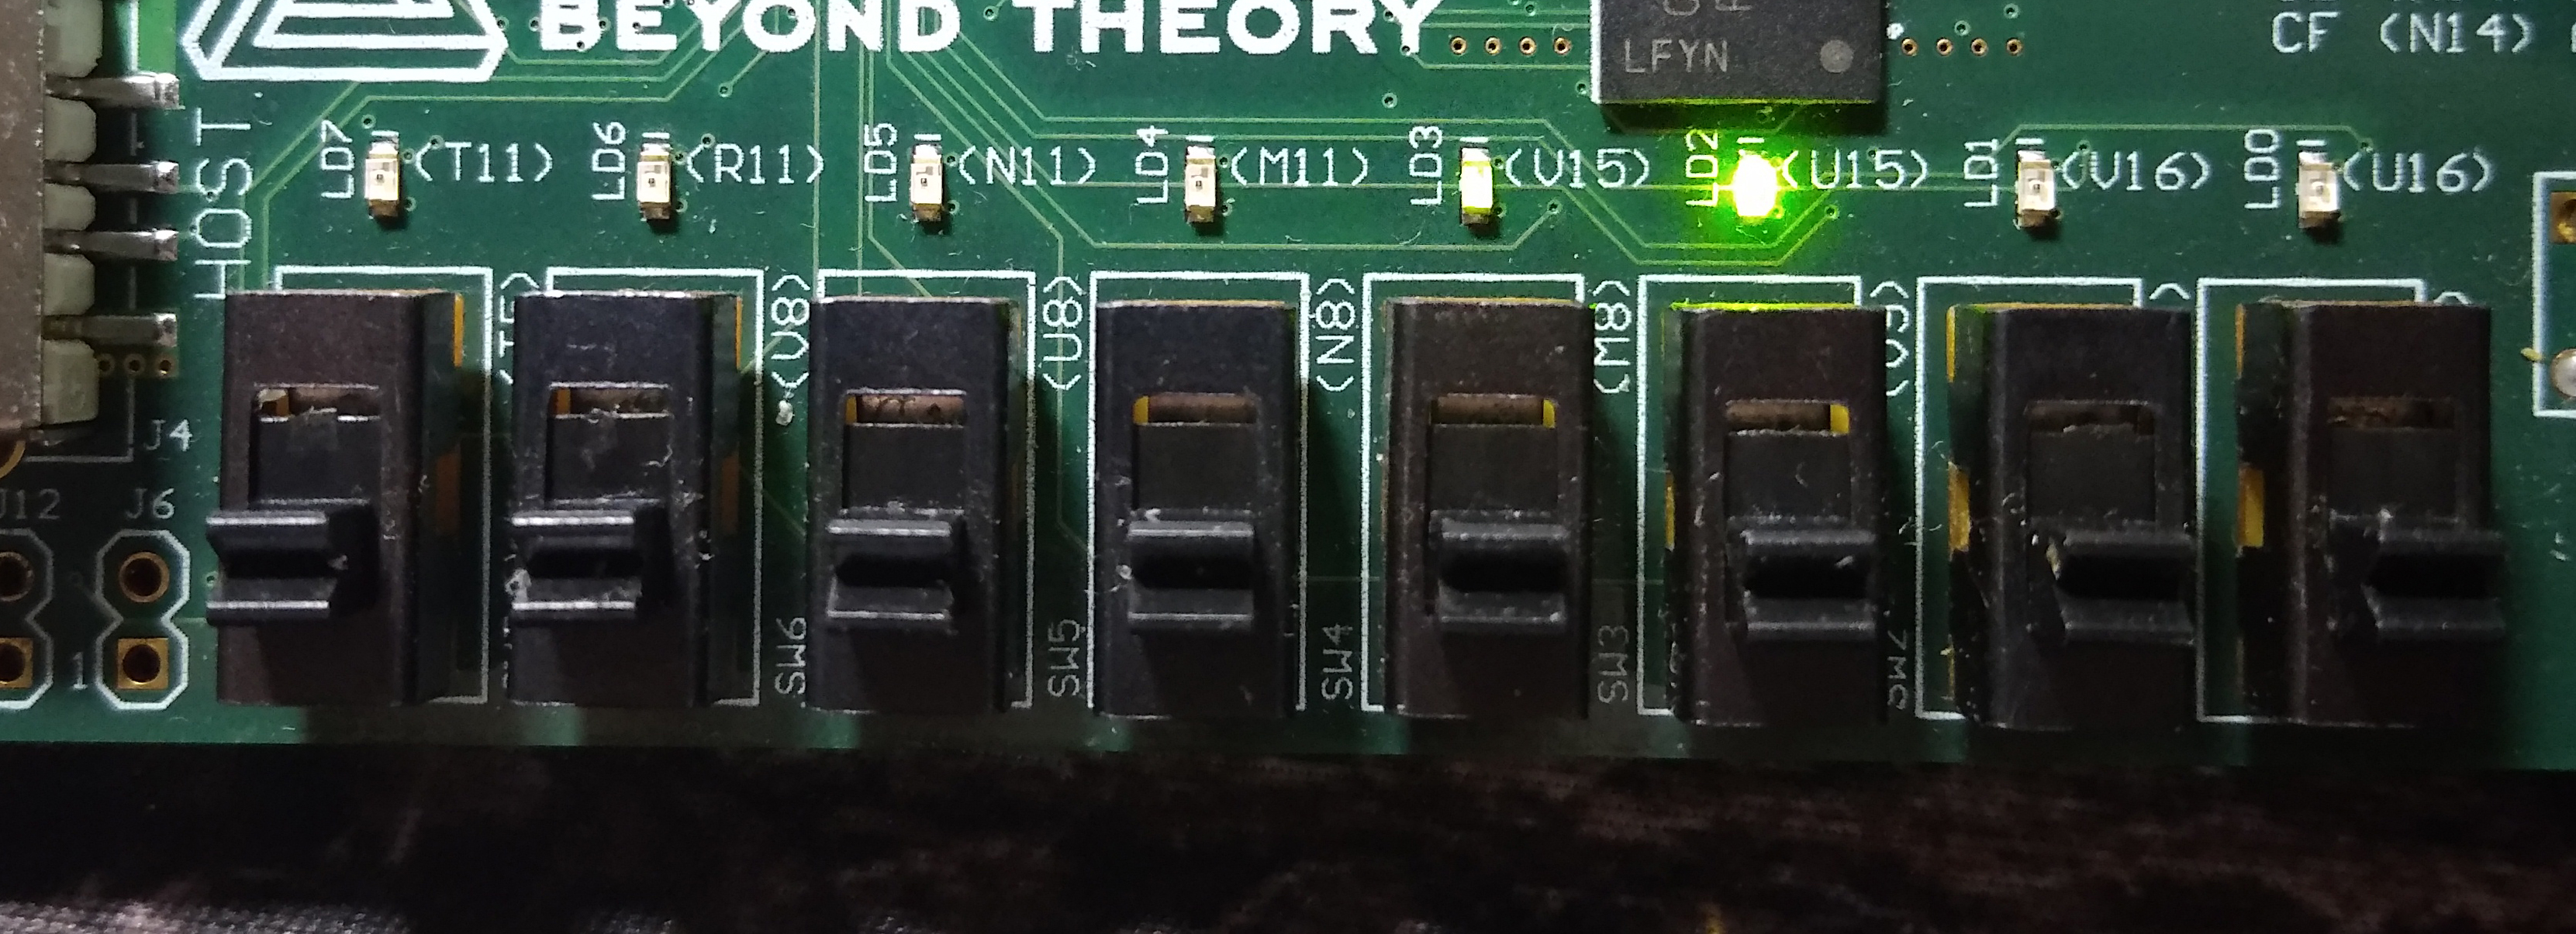
\includegraphics[width=1\linewidth]{report-1-rt-2}
\caption{}
\label{fig:report-1-rt-2}
\end{figure}

        
         %% Exp 1-2
         \section{数码管显示开关按钮状态}
         
         \subsection{实验目的}
         \begin{enumerate}
             \item 熟悉 ISE 软件,会使用ISE软件进行设计和仿真
             \item 学会程序下载
            \end{enumerate}
            
            \subsection{实验内容}
            
            \begin{enumerate}
                \item 创建工程
                \item 设计输入
                \item 综合实现
                \item 进行硬件配置
            \end{enumerate}
            
            \subsection{报告正文}
            
            \subsubsection{实验原理}
            
            Nexys3 开发板上有8个并列排放置的开关 \verb|SW7|~ \verb|SW0|,以及五个按钮。
            8个开关功能表示2位十六进制数。四个按钮则是能表示一位二进制数。并将 \verb|BTND(C9)|作为
            复位开关。%
            \begin{figure}
\centering
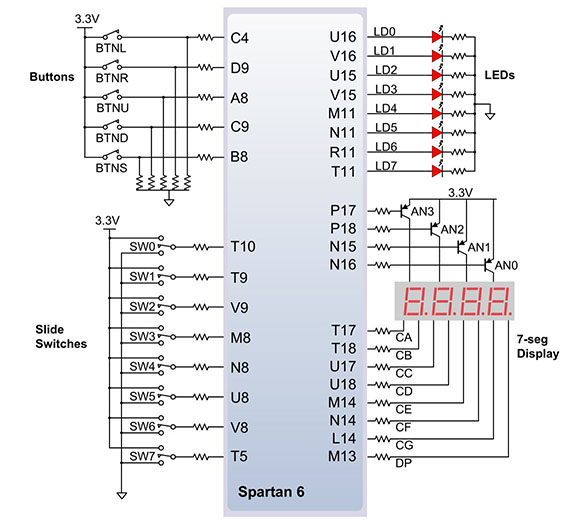
\includegraphics[width=0.7\linewidth]{report-1-io-ports}
\caption{I/O接口}
\label{fig:report-1-io-ports}
\end{figure}
            实验要求4个七段数码管低两位显示开关状态,第三位显示按钮状态。
            根据 图\ref{fig:report-1-io-ports} 所示,\verb|AN0|~\verb|AN3|
            分别是四个数码管的使能信号,其中低电平有效。对于单个数码管,一共有七个段,共阴极。
            下表是关于七段数码管的配置,其中0表示\verb|On|,1表示 \verb|Off|。
            \begin{center}
            \begin{tabular}{c|ccccccc}
                X & a & b & c & d & e & f & g \\ \hline
                0 & 0 & 0 & 0 & 0 & 0 & 0 & 1 \\ 
                1 & 1 & 0 & 0 & 1 & 1 & 1 & 1 \\ 
                2 & 0 & 0 & 1 & 0 & 0 & 1 & 0 \\ 
                3 & 0 & 0 & 0 & 0 & 1 & 1 & 0 \\ 
                4 & 1 & 0 & 0 & 1 & 1 & 0 & 0 \\ 
                5 & 0 & 1 & 0 & 0 & 1 & 0 & 0 \\ 
                6 & 0 & 1 & 0 & 0 & 0 & 0 & 0 \\ 
                7 & 0 & 0 & 0 & 1 & 1 & 1 & 1 \\ 
                8 & 0 & 0 & 0 & 0 & 0 & 0 & 0 \\ 
                9 & 0 & 0 & 0 & 0 & 1 & 0 & 0 \\ 
                A & 0 & 0 & 0 & 1 & 0 & 0 & 0 \\ 
                B & 1 & 1 & 0 & 0 & 0 & 0 & 0 \\ 
                C & 0 & 1 & 1 & 0 & 0 & 0 & 1 \\ 
                D & 1 & 0 & 0 & 0 & 0 & 1 & 0 \\ 
                E & 0 & 1 & 1 & 0 & 0 & 0 & 0 \\ 
                F & 0 & 1 & 1 & 1 & 0 & 0 & 0 \\ 
            \end{tabular} 
            \end{center}         
            
            
            \subsubsection{实验过程}
            
            \paragraph{新建工程}
            
            打开 ISE 14.7之后,选择新建工程,将工程的路径设置好。
            在单击下一步之后,选择 Nexys3 的 Spartan6 XC6SLX16-CS324 芯片对应的配置。硬件描述语言选择 Verilog,其中的设计硬件用的描述语言是 Verilog。
            然后点击下一步之后进入工程信息页面并确认无误之后,点击完成结束工程的创建。
            
            \paragraph{设计输入}
            
            在菜单 \verb|Project| 中选择 \verb|New Source| 创建新的设计,并选择 \verb|Verilog Module| 创建文件。
            
            其中输入的设计文件是
            \begin{lstlisting}[language=Verilog]
`timescale 1ns / 1ps
// Copyright (C) Xilinx
module seg7_display(
input clk,
input reset,
input [7:0] switch,
input [3:0] button,
output [3:0] an,
output [6:0] a_to_g,
output dp
);

reg [3:0] an;
reg [6:0] a_to_g;

wire [1:0] s;
reg [3:0] digit;
wire [3:0] aen;
reg [19:0] clkdiv;

assign dp = 1'b1;
assign s = clkdiv[19:18];	//count every 2.6ms
assign aen = 4'b1111;	//enable all digits

//4位4选1 MUX
always @ (s) begin
case(s)
2'b00: digit = switch[3:0];
2'b01: digit = switch[7:4];
2'b10: digit = button;
default: digit = button;
endcase
end

//7段数码管
always @ (digit) begin
case(digit)
0: a_to_g = 7'b0000001;
1: a_to_g = 7'b1001111;
2: a_to_g = 7'b0010010;
3: a_to_g = 7'b0000110;
4: a_to_g = 7'b1001100;
5: a_to_g = 7'b0100100;
6: a_to_g = 7'b0100000;
7: a_to_g = 7'b0001111;
8: a_to_g = 7'b0000000;
9: a_to_g = 7'b0000100;
'hA: a_to_g = 7'b0001000;
'hB: a_to_g = 7'b1100000;
'hC: a_to_g = 7'b0110001;
'hD: a_to_g = 7'b1000010;
'hE: a_to_g = 7'b0110000;
'hF: a_to_g = 7'b0111000;
default: a_to_g = 7'b0000001;  // 0
endcase
end

//digit select
always @ (s) begin
an = 4'b1111;
if(aen[s] == 1'b1) begin
if(s != 2'b11) begin
an[s] = 1'b0;
end
else begin
an[s] = 1'b1;
end
end
end

//时钟分频器
always @ (posedge clk or posedge reset) begin
if(reset == 1'b1) begin
clkdiv <= 0;
end
else begin
clkdiv <= clkdiv + 1'b1;
end
end

endmodule
            \end{lstlisting}
            \paragraph{综合与实现}
            
            在左侧的 \verb|Design| 面板中下方中 双击 \verb|Synthesize-XST| 开始综合过程。
            
            
            在左侧的 \verb|Design| 面板中的 \verb|Hierarchy| 中选中创建的 HDL 源文件,在下方的双击 \verb|View RTL Schematic| 查看电路。
            
        \begin{figure}
            \centering
            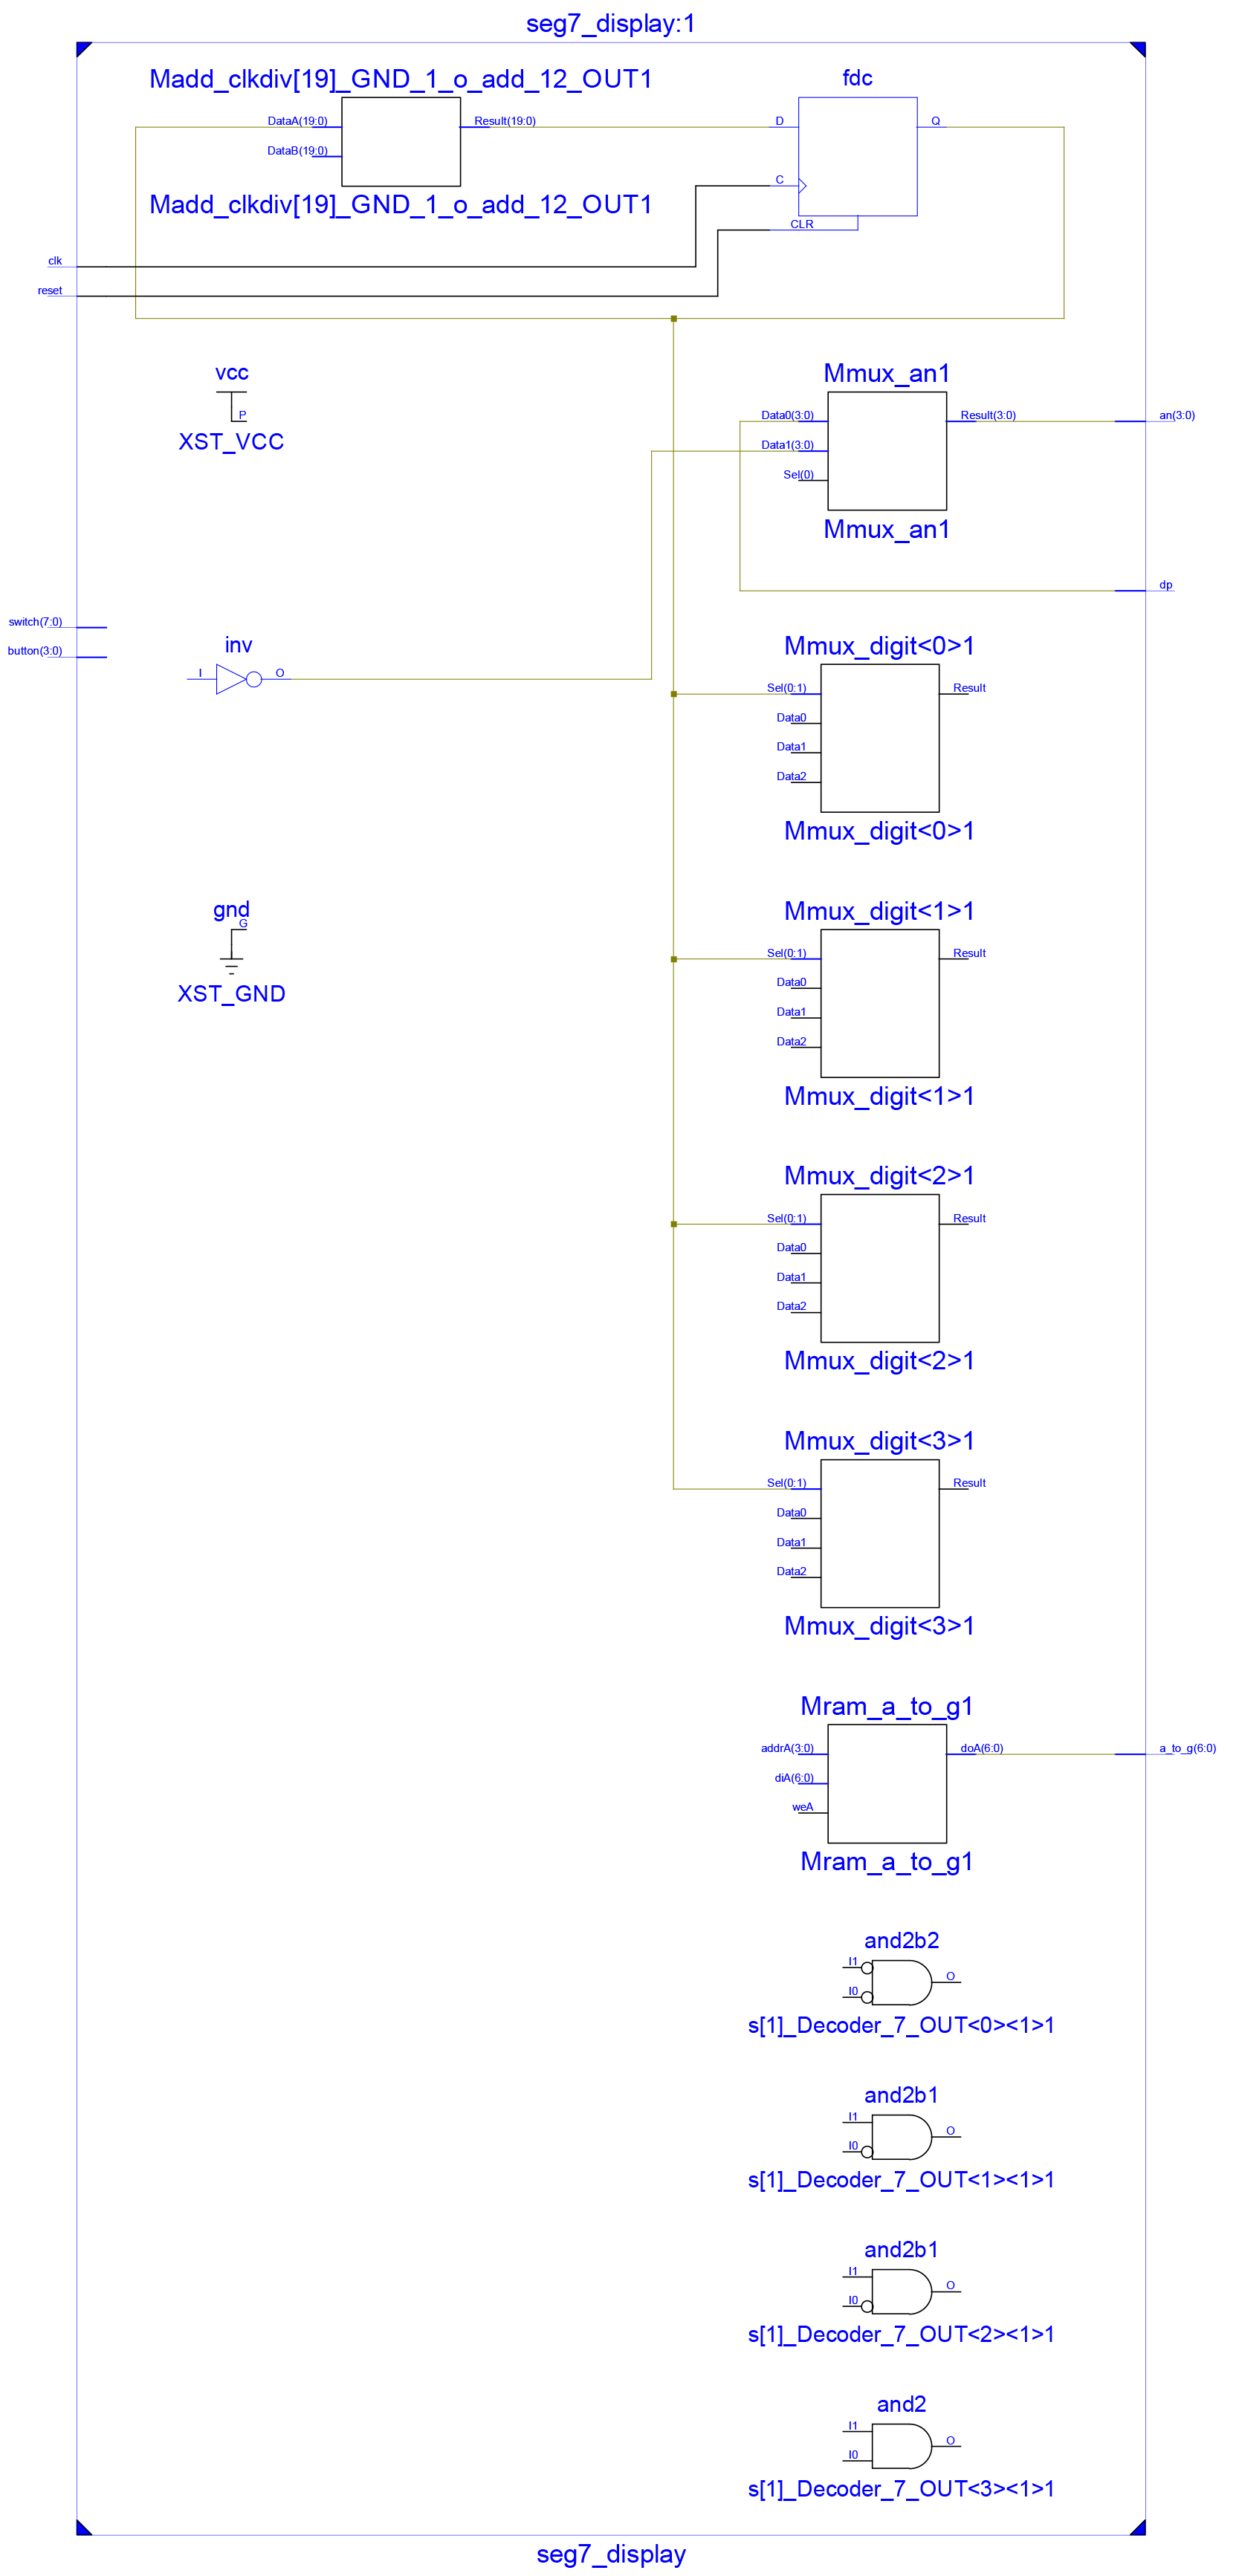
\includegraphics[width=1\linewidth]{report1-circiut-2.jpg}
            \caption[Circuit]{}
            \label{fig:report1-circiut-2}
        \end{figure}
        
        之后添加用户约束文件,这个文件使得器件脚针与外围设备可以绑定,链接。
        添加的方式可以在 \verb|Design| 面板中找到 带有 \verb|Pre| 前缀的 \verb|PlanAhead| 中配置脚针。或者为工程添加用户约束文件。
        
        \begin{figure}
\centering
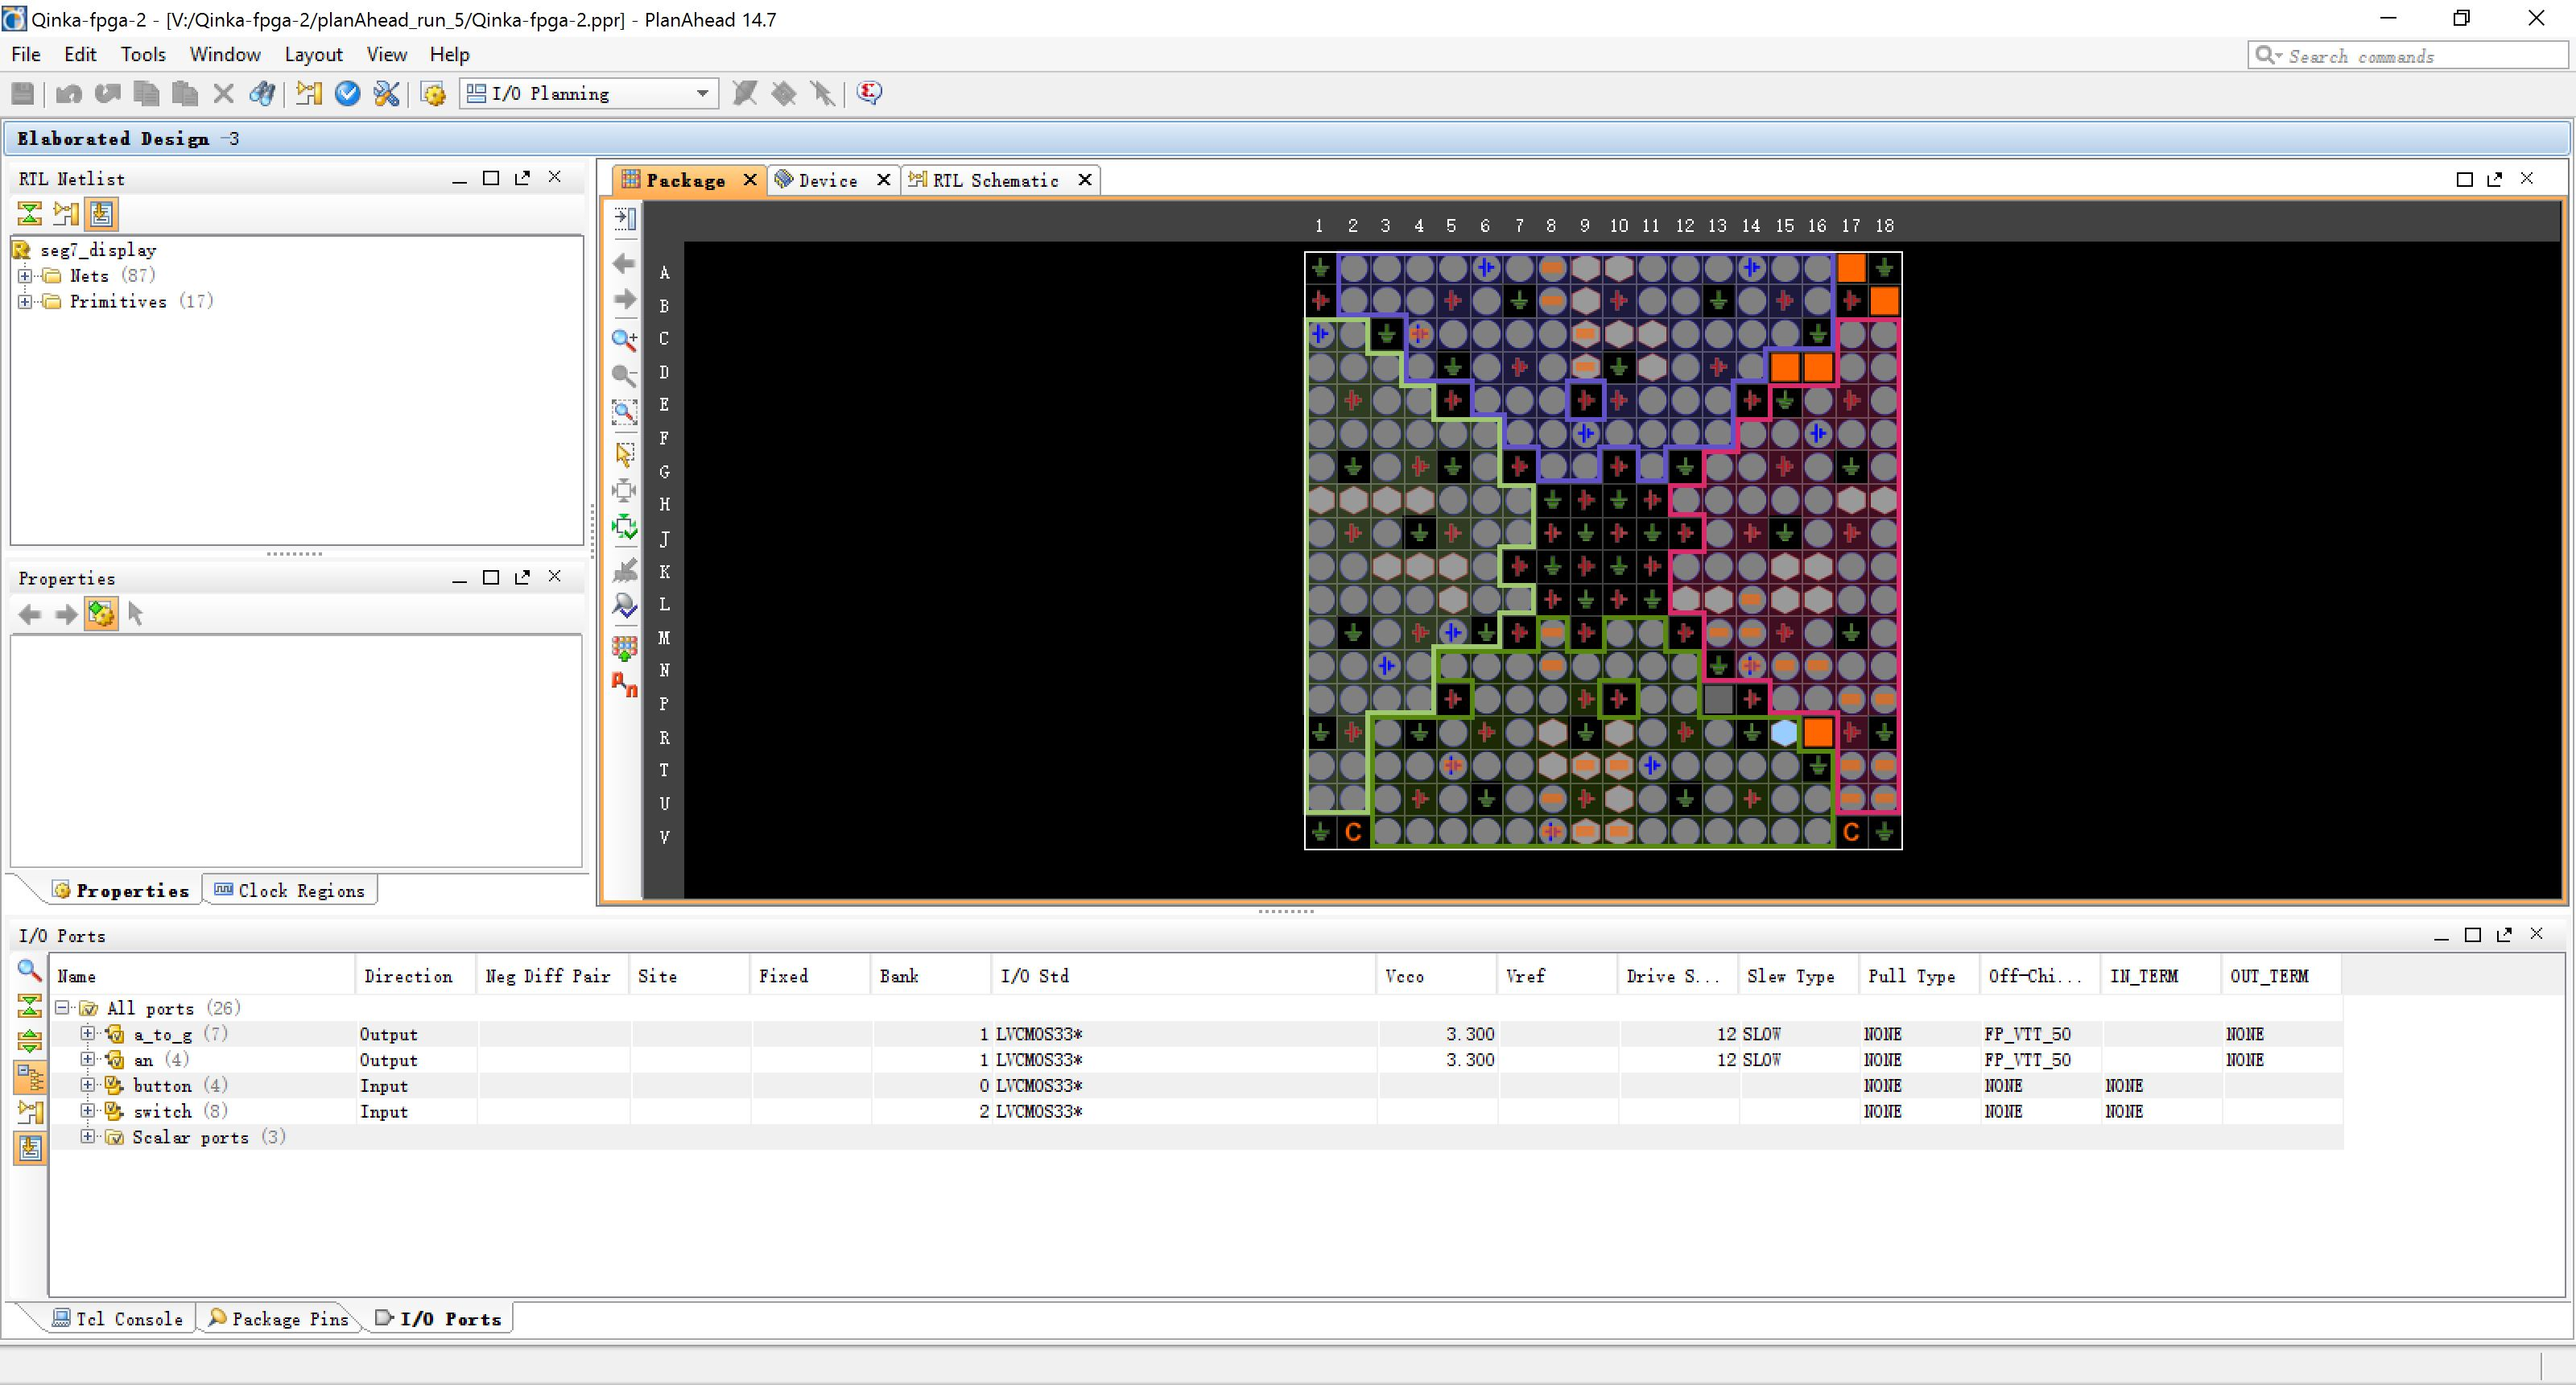
\includegraphics[width=1\linewidth]{report-1-io-ports-2}
\caption{}
\label{fig:report-1-io-ports-2}
\end{figure}

        
        用户约束文件的内容大致是配置脚针(site) 与外围设备的链接配置。
        
        \begin{lstlisting}
NET "a_to_g[6]" IOSTANDARD = LVCMOS33;
NET "a_to_g[5]" IOSTANDARD = LVCMOS33;
NET "a_to_g[4]" IOSTANDARD = LVCMOS33;
NET "a_to_g[3]" IOSTANDARD = LVCMOS33;
NET "a_to_g[2]" IOSTANDARD = LVCMOS33;
NET "a_to_g[1]" IOSTANDARD = LVCMOS33;
NET "a_to_g[0]" IOSTANDARD = LVCMOS33;
NET "an[3]"     IOSTANDARD = LVCMOS33;
NET "an[2]"     IOSTANDARD = LVCMOS33;
NET "an[1]"     IOSTANDARD = LVCMOS33;
NET "an[0]"     IOSTANDARD = LVCMOS33;
NET "button[3]" IOSTANDARD = LVCMOS33;
NET "button[2]" IOSTANDARD = LVCMOS33;
NET "button[1]" IOSTANDARD = LVCMOS33;
NET "button[0]" IOSTANDARD = LVCMOS33;
NET "switch[7]" IOSTANDARD = LVCMOS33;
NET "switch[6]" IOSTANDARD = LVCMOS33;
NET "switch[5]" IOSTANDARD = LVCMOS33;
NET "switch[4]" IOSTANDARD = LVCMOS33;
NET "switch[3]" IOSTANDARD = LVCMOS33;
NET "switch[2]" IOSTANDARD = LVCMOS33;
NET "switch[1]" IOSTANDARD = LVCMOS33;
NET "switch[0]" IOSTANDARD = LVCMOS33;
NET "clk"       IOSTANDARD = LVCMOS33;
NET "dp"        IOSTANDARD = LVCMOS33;
NET "reset"     IOSTANDARD = LVCMOS33;

NET "switch[7]" LOC = T10;
NET "switch[6]" LOC = T9;
NET "switch[5]" LOC = V9;
NET "switch[4]" LOC = M8;
NET "switch[3]" LOC = N8;
NET "switch[2]" LOC = U8;
NET "switch[1]" LOC = V8;
NET "switch[0]" LOC = T5;
NET "button[0]" LOC = D9;
NET "button[1]" LOC = B8;
NET "button[2]" LOC = A8;
NET "button[3]" LOC = C4;
NET "an[0]"     LOC = N16;
NET "an[1]"     LOC = N15;
NET "an[2]"     LOC = P18;
NET "an[3]"     LOC = P17;
NET "a_to_g[0]" LOC = L14;
NET "a_to_g[1]" LOC = N14;
NET "a_to_g[2]" LOC = M14;
NET "a_to_g[3]" LOC = U18;
NET "a_to_g[4]" LOC = U17;
NET "a_to_g[5]" LOC = T18;
NET "a_to_g[6]" LOC = T17;
NET "clk"       LOC = V10;
NET "dp"        LOC = M13;
NET "reset"     LOC = C9;
        \end{lstlisting}
        
        然后执行的步骤是实现。这个步骤中会执行翻译、映射、与布局布线。双击
        \verb|Implement Design| 自动执行上述步骤。
        
        \paragraph{器件配置}
        
        配置器件之前首先需要进行的是生成对应的配置文件。在 \verb|Design| 面板中
        的 \verb|Generate Programming File|  双击之后会自动生成 二进制比特的配置文件。
        之后将开发版通过USB链接到电脑后。双击 \verb|Configure Target Device| 配置设备。
        
        对FPGA配置编程的时候,会打开一个窗口,初始化链之后可添加设备。然后将生成的配置文件写入
        FPGA 中。然后就可以通过搬动开关活着按下按钮测试显示的内容了。
        
        \begin{figure}
\centering
\includegraphics[width=1\linewidth]{report-1-rt-3}
\caption{}
\label{fig:report-1-rt-3}
\end{figure}
\begin{figure}
\centering
\includegraphics[width=1\linewidth]{report-1-rt-4}
\caption{}
\label{fig:report-1-rt-4}
\end{figure}


\end{document}